%! TEX root = ../../master.tex
\lecture[Alternative MST formulations. Submodularity. Deriving Kruskal from $\LP$.]{Do 12 May 2022}{Submodularity}
\begin{definition}
    Given a graph $G=(N,E)$ and cost vector $c \in \realnum^E$. Finding a spanning tree $T$
    such that $c(T)$ is minimal is called $\vocab{Minimal Spanning Tree}$ problem, short $\MST$.
\end{definition}
\begin{recall}
    In ADM1 we learned that we can use \vocab{Kruskal's algorithm} to find a $\MST$ in polynomial time.
    Kruskal sorted the edges and added edges in this order if it wouldn't create a cycle.

    On the other hand, there is also an $\LP$ formulation:
    \begin{mini*}{x}{c^Tx}{}{}
        \addConstraint{x(\gamma(K))}{\leq |K|-1, \quad}{K \subsetneq N}
        \addConstraint{x(E)}{= n-1}
        \addConstraint{x}{\geq 0}
    \end{mini*}
\end{recall}
Tom doesn't like the $\LP$ formulation, though, because
\begin{enumerate}
    \item "$\min$" and "$\leq$" just feel wrong,
    \item rather than $x(\gamma(K))$, we should use $x(S)\leq ?$ for $S \subseteq E$.
\end{enumerate}
We can circumvent this problems with following $\LP$, for some $M >> \max_i w_i$ and $w = M - c$, and some magic function $r$:
\begin{mini}{w}{w^Tx}{}{} \label{eq:kruskal_alt}
    \addConstraint{x(S)}{\leq r(S), \quad}{S \subseteq E}
    \addConstraint{x}{\geq 0}
\end{mini}
Let's have a closer look at $r(S)$, and define it as the maximum number of edges we can choose in $S$
without creating a cycle.

Let's also define $cc(S)$ as the number of \vocab{connected components} in $(N,S)$.
\begin{theorem} \label{thm:cc-r-function}
    For a graph $G=(N,E)$ it holds that
    $r(S)=n - cc(S)$.
\end{theorem}
\begin{proof}
    Let $C_1,...,C_k$ be node sets of connected components of $(N,S)$, meaning $cc(S)=k$.
    Note that $\sum_i |C_i|=n$.
    Furthermore, we can choose at most $|C_i|-1$ acyclic edges per component $C_i$ by choosing any spanning tree.
    Thus,
    \begin{align*}
        r(S) & =\ \text{maximum acyclic edges in $(N,S)$}      \\
             & =\sum_i (\text{maximum acyclic edges in $C_i$}) \\
             & =\sum_i |C_i|-1 = n-k = n-cc(S).
    \end{align*}
\end{proof}
\begin{example} Consider following graph:
    \\
    \begin{minipage}{\textwidth}
        \centering
        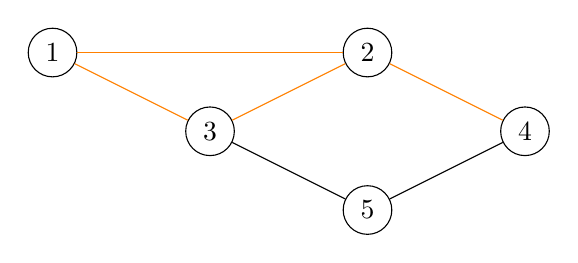
\begin{tikzpicture}
            \begin{scope}[every node/.style={circle, draw}]

                \node (1) at (0,0) {$1$};
                \node (2) at (4,0) {$2$};
                \node (3) at (2,-1) {$3$};
                \node (4) at (6,-1) {$4$};
                \node (5) at (4,-2) {$5$};

                \path[draw=orange] (1) edge (2);
                \path[draw=orange] (2) edge (3);
                \path[draw=orange] (1) edge (3);
                \path[draw=orange] (2) edge (4);
                \path (5) edge (4);
                \path (5) edge (3);
            \end{scope}
        \end{tikzpicture}
        % \captionof{figure}{A graph with $S$ colored orange}
    \end{minipage}
    For the \textcolor{orange}{drawn $S$}, it holds $cc(S)=2$, namely $\{1,2,3,4\}$ and $\{5\}$, and thus $r(S)=5-2=3$.
\end{example}
We can construct the dual of \eqref{eq:kruskal_alt}:
\begin{mini}{y_S}{r(S)y_S}{}{} \label{eq:kruskal_dual}
    \addConstraint{\sum_{S: e \in S}y_S}{\geq w_e, \quad}{\forall e \in E}
    \addConstraint{y}{\geq 0}
\end{mini}
\begin{warning}
    Our original $\LP$ had $2^n$ constraints, which means our dual has $2^n$ variables. Even the data $r(S)$ cannot be written down in polynomial time!
\end{warning}
This means we need to think about $r(S)$ a little bit more. Consider a set $R$ and edge $e\in E$ with $R \subset S \subset S + e$.
The so-called \vocab{marginal cost} of adding $e$ to $R$ is $r(R+e)-r(R) \in \{0,1\}$. Same goes for $S$.

\begin{definition}
    For a set $M$, let $r : \mathcal P(M) \rightarrow \realnum^+_0$ be a function.
    If the marginal costs are non-decreasing for $R \subset S$ for the same edge, i.e.
    \begin{align*}
        r(S+e)-r(S) \leq r(R+e) - r(R),
    \end{align*}
    then we call $r$ \vocab{submodular}.
\end{definition}
\begin{theorem}
    Our acyclic-$r(S)$ is submodular.
\end{theorem}
\begin{proof}
    It suffices to show that $r(S+e)-r(S)=1$ and $r(R+e)-r(R)=0$ cannot happen.
    Note that the connected components of $R$ are subsets of connected components of $S$. Thus, if we add an edge $e$ that connects two
    connected components, it also connects two components of $R$. By \autoref{thm:cc-r-function}, this is the only way $r(S)$ increases by one,
    but also forces $r(R)$ to increase.
\end{proof}
There is also an equivalent definition of submodularity:
\begin{theorem} \label{thm:submodularity}
    A function $r : \mathcal{P}(M) \rightarrow \realnum$ is \vocab{submodular} iff for all $S,R \subseteq E$
    \begin{align*}
        r(S)+r(R) \geq r(S\cap R) + r(S \cup R).
    \end{align*}
\end{theorem}
\begin{proof}
    See \autoref{ex:5.2}.
\end{proof}
Now let's try to derive Kruskal from our $\LP$s \eqref{eq:kruskal_alt} and \eqref{eq:kruskal_dual}:
\begin{lemma}
    Suppose $x^*,y^*$ are optimal in their corresponding $\LP$s  \eqref{eq:kruskal_alt} and \eqref{eq:kruskal_dual}.
    Among the dual optimal
    solution let $y^*$ be the one with $y^*=\sum_{S\subset E}(y_S)^2$ (notice the square!).

    Then for $R,S \subset E$, if $y_R^*, y_S^* > 0$, it follows that either $R \subset S$ or $S \subset R$.
    We call this property \vocab{nested}.
\end{lemma}
\begin{proof}
    Assume $y_R^*, y_S^* > 0$, but are not nested.
    Let $\eps = \min(y_R^*,y_S^*0) >0$ and
    \begin{align*}
        y_Q^\prime = \begin{cases}
                         y_Q^*- \eps, & \text{if } Q= R \OR Q=S,               \\
                         y_Q^*+ \eps, & \text{if } Q= R \cup S \OR Q=R \cap S, \\
                         y_Q^*,       & \text{otherwise}.                      \\
                     \end{cases}
    \end{align*}
    Then $y^\prime$ is still feasible, because the $\eps$ cancel out, since $R \cup S$ and $R \cap S$ must be new sets,
    and every edge is either in all four sets, no set, or exactly one of $R,S$ and $R\cup S,R\cap S$ each.
    The choice of $\eps$ ensures $y^\prime \geq 0$.

    Now have a look how the objective function changes and consider the difference given by:
    \begin{align*}
        \eps (\underbrace{r(R \cap S) + r(R \cup S) - r(R) - r(S)}_{\leq 0\ \text{by submodularity}})
    \end{align*}
    We cannot get cheaper though, because we were already optimal. Therefore,  $y^\prime$ is also an optimal dual solution, but
    \begin{align*}
        \sum_S(y_S^\prime)^2 < \sum_S(y^*_S)^2
    \end{align*}
    is a contradiction! (One can check this by tedious calculations.)
\end{proof}
Consider $\mathcal{J} \coloneqq \{S \subseteq E \mid y_S^* > 0\}$.
Because of previous lemma we can build a chain of elements of $\mathcal J$:
\begin{align*}
    S_1 \subset ... \subset S_m, \quad |S_i|=i.
\end{align*}
If length $m$ is not possible, add some $y^*_S=0$ sets.
Thus, using this $S$ as a basis yields following system:
% \begin{align*}
\[
    \begin{pNiceMatrix}[first-row, first-col]
               & S_1    & S_2    & S_3 & \Cdots & S_m    \\
        e_1    & 1      & \Cdots &     &        & 1      \\
        e_2    & 0      & \Ddots &     &        & \Vdots \\
        e_3    & \Vdots & \Ddots &     &        &        \\
        \Vdots &        &        &     &        &        \\
        e_m    & 0      & \Cdots &     & 0      & 1      \\
    \end{pNiceMatrix}
    \begin{pNiceMatrix}
        y_{S_1}^* \\
        y_{S_2}^* \\
        y_{S_3}^* \\
        \Vdots    \\
        y_{S_m}^*
    \end{pNiceMatrix}
    =\begin{pNiceMatrix}
        w_{e_1} \\
        w_{e_2} \\
        w_{e_3} \\
        \Vdots  \\
        w_{e_m}
    \end{pNiceMatrix}
    % \end{align*}
\]
Note the basis matrix has continuous ones property (and thus being totally unimodular by \autoref{thm:cop-is-tu}), and is
an upper triangular matrix, meaning the resulting equation system is easy to solve.
In fact, substituting yields
\begin{align*}
    y^*_{S_m}     & =w_{e_m}           \\
    y^*_{S_{m-1}} & =w_{e_m-1}-w_{e_m} \\
                  & \vdots             \\
    y^*_{S_{1}}   & =w_{e_1}-w_{e_2}
\end{align*}
So, for this $y^*$ to be feasible (i.e. non-negative), the edges need to be ordered by weight, just like in Kruskal!
Furthermore, for every edge $e_k \in E$ it holds
\begin{align*}
    \sum_{S: e_k \in S}y_S^* & = \sum_{i=k}^m y_{S_i}^*    \\
                             & =\sum_{i=k}^m w_i - w_{i+1} \\
                             & = w_{e_k},
\end{align*}
concluding feasibilty according to \eqref{eq:kruskal_dual}.

On the other hand, we can simply derive a primal optimal basis:
\[
    \begin{pNiceMatrix}[first-row, first-col]
               & e_1    & e_2    & e_3    & \Cdots & e_m    \\
        S_1    & 1      & 0      & \Cdots &        & 0      \\
        S_2    & \Vdots & \Ddots & \Ddots &        & \Vdots \\
        S_3    &        &        &        &        &        \\
        \Vdots &        &        &        &        & 0      \\
        S_m    & 1      & \Cdots &        &        & 1      \\
    \end{pNiceMatrix}
    \begin{pNiceMatrix}
        x_{e_1}^* \\
        x_{e_2}^* \\
        x_{e_3}^* \\
        \Vdots    \\
        x_{e_m}^*
    \end{pNiceMatrix}
    =\begin{pNiceMatrix}
        r(S_1) \\
        r(S_2) \\
        r(S_3) \\
        \Vdots \\
        r(S_m)
    \end{pNiceMatrix}
\]
Analoguous, we get
\begin{align*}
    x_{e_i}^* & = r(S_i) - r(S_{i-1})               \\
              & = r(S_{i-1}+e_i)-r(S_i) \in \{0,1\}
\end{align*}
which represents the edge addition step, and assures feasibilty of \eqref{eq:kruskal_alt}!

It remains to be shown that our constructed solutions are indeed optimal.
Using strong duality, we see
\begin{align*}
    \sum_{i=1}^m w_i x_{e_i}^* & = \sum_{i=1}^m w_i (r(S_i) - r(S_{i-1})) \\
                               & = \sum_{i=1}^m r(S_i)(w_i - w_{i+1})     \\
                               & = \sum_{i=1}^m r(S_i)y_{S_i}^*
\end{align*}
\begin{conclusion}
    Using only a submodular function and $\LP$s, we constructed an algorithm that
    solves $\MST$. In particular, no special facts about trees etc. were used.
\end{conclusion}